\startchapter{Challenges with Copilot}
\label{chapter:methodology}

\section{Introduction}
Useful \cct{} should always suggest recommended coding best practices in its first suggestion. In this chapter, we test if Copilot suggests the recommended ways sampled from popular sources.
We begin by explaining the current challenges with \cct{} like Copilot, showing recent research works on common problems faced with using Copilot and the motivation to find the limitations of current \cct{} like Copilot~(section~\ref{challenges}).

In section~\ref{methodology}, we explain our approach to \textbf{RQ-1} (What are the current boundaries of \cct{}?). 
We describe our sampling approach to collecting Pythonic idioms~(section~\ref{sampling}) and best practices in JavaScript~(section~\ref{smells:sampling}). We then describe the input given to Copilot for triggering the generation of code suggestions~(section~\ref{input}).
Finally, we explain our evaluation method to compare Copilot suggestions to the recommended practices~(section~\ref{evaluation}).

In section~\ref{results}, we present our results on performance of Copilot in suggesting recommended practices for 50 different coding scenarios~(25 pythonic idioms + 25 code smells), which answers \textbf{RQ-1.1} (How do \cct{} manage programming idioms?), and \textbf{RQ-1.2} (How do \cct{} manage to write non-smelly code?).
We observe that Copilot had the recommended practices in its top 10 suggestions for 18 out of 50 coding scenarios~(36\% of all tests performed).

% In section~\ref{methodology}, we describe our sampling approach to collecting python idioms and the evaluation method used to compare Copilot suggestions to the optimal way listed in python idioms. In section~\ref{secidioms}, we show the results of the study comparing Copilot suggestions and idioms in python programming language. We observe that Copilot performs poorly in suggesting the optimal way in its suggestions. 

% Having identified the performance of current \cct{} like Copilot on detecting and suggesting common patterns like language idioms in chapter~\ref{chapter:idioms}, in this chapter we test if Copilot suggests code that follows code review standards.
% We begin by explaining our approach to \textbf{RQ-1.1} (How do \cct{} manage to write non-smelly code?). To achieve this, we conduct an exploratory study to find if \cct{} tools like Copilot suggest the best practices based on code review standards in their suggestions. 

% In section~\ref{smells:methodology}, we describe our sampling approach to collecting best practices in javascript and the evaluation method used to compare Copilot suggestions to the best practices listed in coding style and code review standards. 
% In section~\ref{bp}, we show the results of the study comparing Copilot suggestions and code review standards in javascript.

\section{Background \& Motivation}
\label{challenges}
Code completion tools are very useful but are often limited to the generation of single elements (e.g., method calls and properties) and the usage of templates. 
Furthermore, too many recommendations can decrease the usefulness of the tool~\cite{Proksch2015}. 
\cct{} must be accurate with its code suggestions while minimizing the number of different code suggestions recommended to the user.

Copilot can make simple coding mistakes, such as not allowing for an empty array in a sort routine\footnote{all examples are documented in our \repl{}.}. Copilot does not understand security vulnerabilities, so it will suggest code that allows for a \textsf{log4shell} vulnerability\footnote{\url{https://www.wiz.io/blog/10-days-later-enterprises-halfway-through-patching-log4shell/}}, or common SQL injection attacks. A recent study by Pearce et al.~\cite{copilot_security} showed that approximately 40\% of the code suggested by Copilot is vulnerable when tested on 89 different scenarios for Copilot to complete.
Some of these basic programming challenges have been already documented and are, we suspect, very much under consideration by the corporate teams behind Copilot and Codex. 
Since these tools are trained on existing software source code and training costs are expensive, several classes of errors have been discovered, which follow from the presence of these same errors in public (training) data.
Similarly, concerns have been raised about Copilot license compliance and copyright violation~\cite{code_clone}; with similar input data, Copilot suggests identical code to existing code on GitHub, which may be under copyright. 
As it is trained on public data collected in May 2020 from 50 million public repositories on GitHub~\cite{copilot}, any code uploaded after that date is absent in the knowledge base of Copilot. 
% The training data for Copilot was collected in May 2020 from 50 million public repositories on GitHub~\cite{copilot}. 
%It does not have any data uploaded to GitHub after that date and any data from useful sources like documentation and Stack Overflow to improve its suggestions from commonly occurring bugs.

Karampatsis et al.~\cite{github_bugs} showed that for the 1000 most popular open-source Java repositories on GitHub, there is a frequency of one single statement bug per 1600-2500 lines of code and about 33\% of all the bugs match a set of 16 bug templates. 
So, any software flaws present in large numbers on GitHub will tend to dominate the learning of the model.
But these challenges are not surprising and have straightforward fixes. These fixes might include better data engineering and filtering to remove known problems, like a filter introduced by GitHub to suppress code suggestions containing code that matches public code on GitHub, although the exact filtering process has not been publicly disclosed.

Similarly, it seems viable to conduct security scans or linting runs before suggesting removing obvious problems like SQL injection. 
Clone detection techniques can help find places where code violates the copyright. 
Better machine learning approaches, using active learning or fine-tuning, might help learn local lessons~\cite{Menzies2013} for customization in the case of identifier naming or formatting.
In most of these cases, good tools exist already for this. 

Although these are clearly challenges, Copilot seems already to be on its way to fixing them, like a filter introduced by GitHub to suppress code suggestions containing code that matches public code on GitHub. 
However, what is more difficult to envision are the problems that are harder to fix because straightforward corrections may not exist, and rules for finding problems are more challenging to specify than those in smell detectors or linters~\cite{Ernst2017} like language idioms and code smells.

Developers often discuss software architecture and actual source code implementations in online forums, chat rooms, mailing lists, or in person. 
Programming tasks can be solved in more than one way. 
The best way to proceed can be determined based on case-specific conditions, limits, and conventions. Strong standards and a shared vocabulary make communication easier while fostering a shared understanding of the issues and solutions related to software development.
However, this takes time and experience to learn and use idiomatic approaches~\cite{Alexandru2018}.

\cct{} can help steer users into using more idiomatic approaches with its code suggestions or vice-versa.
This makes it crucial to find the boundaries of \cct{} like Copilot~(\textbf{RQ 1}) and create a clear understanding of where can we use \cct{} like Copilot and where should the user be vigilant in using \cct{} code suggestions.
To achieve this, we conduct an exploratory study to find if \cct{} tools like Copilot suggest the recommended best coding practices in their suggestions.
\section{Methodology}
\label{methodology}
In this section, We explain the methodology we used to address \textbf{RQ-1} (What are the current boundaries of \cct{}?). We perform our experiments Copilot suggestions on Pythonic Idioms~(section~\ref{idioms}) and code smells in JavaScript~(section~\ref{smells}).

Additionally, we explain how 25 coding scenarios for Pythonic idioms~(section~\ref{smells:sampling}) and code smells in JavaScript~(section~\ref{sampling}) were sampled.
Finally, we discuss how the input is shaped to trigger Copilot to generate code suggestions~(section~\ref{input}) and how Copilot suggestions are evaluated (section~\ref{evaluation}).
The following analysis was carried out using the Copilot extension in Visual Studio Code. We use the most recent stable release of the Copilot extension available at the time of writing~(version number 1.31.6194) in Visual Studio Code.

\subsection{Pythonic Idioms}
\label{python}
A software language is more than just its syntax and semantics; it is also a set of known effective ways to address real-world issues using it. 
To answer \textbf{RQ-1.1} (How do \cct{} manage programming idioms?),
we chose Python, one of the most popular programming languages, because Copilot's base model Codex performs best in Python~\cite{copilot}.  

The definition for the term \emph{Pythonic} in Python found in official Python glossary\footnote{\url{https://docs.python.org/3/glossary.html\#term-pythonic}} as follows:

\begin{quote}
    An idea or piece of code follows the most common idioms of the Python language rather than implementing code using concepts common to other languages. For example, a common idiom in Python is to loop over all elements of an iterable using a for statement. Many other languages do not have this construct, so people unfamiliar with Python sometimes use a numerical counter instead, instead of the cleaner, pythonic method.
\end{quote}

This definition indicates a broad meaning, referring to both concrete code and also \emph{Ideas} in a general sense. Many Python developers argue that coding the \emph{pythonic way} is the most accepted way to code by the Python community~\cite{Alexandru2018}. 
We consider an \emph{idiom} to be any reusable abstraction that makes Python code more readable by shortening or adding syntactic sugar. Idioms can also be more efficient than a basic solution, and some idioms are more readable and efficient.
The pythonicity of a piece of code stipulates how concise, easily readable, and generally good the code is. This concept of pythonicity, as well as the concern about whether code is pythonic or not, is notably prevalent in the Python community.

We sampled idioms from the work of Alexandru et al.~\cite{Alexandru2018}, and Farook et al.~\cite{idioms}, which identified idioms from presentations given by renowned Python developers that frequently mention idioms, e.g., Hettinger~\cite{hettinger} and Jeff Knupp~\cite{knupp} and 
popular Python books, such as ``Pro Python''~\cite{Alchin2010}, ``Fluent Python''~\cite{fluent}, ``Expert Python Programming''~\cite{expert}.


\subsubsection{Sampling Approach}
\label{sampling}
We sampled the top 25 popular pythonic idioms found in open source projects based on the work of Alexandru et al.~\cite{Alexandru2018}, and Farook et al.~\cite{idioms}.
The decision to sample \emph{most popular} pythonic idioms is taken to give the best chance for Copilot to suggest the pythonic way as its top suggestion. As a result, Copilot will have the pythonic way more frequently in its training data and more likely to suggest the pythonic way in its suggestions.
However, Copilot is closed source, and we cannot determine if the frequency of code snippets in training data affects Copilot's suggestions. Research by GitHub shows that Copilot can sometimes recite from its training data in ``generic contexts"\footnote{\url{https://github.blog/2021-06-30-github-copilot-research-recitation/}}, which may lead to potential challenges like license infringements~(shown in section~\ref{challenges}). 
Sampling the most frequently used idioms will also help understand if Copilot can recite idioms present in its training data~(GitHub public repositories), which is the ideal behavior for \cct{}.

\subsection{Code Smells}
\label{smells}
A standard style guide is a set of guidelines that explain how code should be written, formatted and organized. 
Using a style guide ensures that code can be easily shared among developers. As a result, any new developer may immediately become familiar with a specific piece of code and write code that other developers will quickly and easily comprehend.
A good \cct{} tool should only suggest code consistent with coding style and pass code reviews by humans. 

To answer \textbf{RQ-1.2} (How do \cct{} manage to suggest non-smelly code?), we chose JavaScript to generalize our experiments with Copilot. 
We relied on the AirBNB javascript coding style guide~\cite{airbnb_code}, a widely used coding style and code review standard introduced in 2012, described as a ``primarily reasonable approach to JavaScript''~\cite{airbnb_code}.

% \section{Methodology}
% \label{smells:methodology}
% In this Section, we explain the methodology we used to address \textbf{RQ-1.2} (How do \cct{} manage to suggest non-smelly code?), including how the best practices were sampled (section~\ref{smells:sampling}), what was the input for Copilot (section~\ref{smells:input}) and how the Copilot suggestions are evaluated (section~\ref{smells:evaluation}). All of the following analysis was carried out using Copilot extension in visual studio code. We use the most recent stable release of Copilot extension (version number 1.30.6165) in visual studio code.

\subsubsection{Sampling Approach}
\label{smells:sampling}
The AirBNB JavaScript coding style guide~\cite{airbnb_code} contains a comprehensive list of best practices covering nearly every aspect of javascript coding like objects, arrays, modules, and iterators. However, it also includes project-specific styling guidelines like naming conventions, commas, and comments.
Since we are testing Copilot for widely accepted best practices and not project-specific styling in JavaScript. 
We sampled 25 best practices from the AirBNB JavaScript coding style guide~\cite{airbnb_code}, 
which were closer to the design level rather than the code level. For example, selecting logging practices as a sample coding standard rather than trailing comma use in javascript as a coding standard. 
This sampling approach ensures Copilot is not tested against personalized styling guidelines of one specific project or a company. In contrast, our goal for Copilot here is to be tested against practices that bring performance or efficiency to the code base.

% \subsection{Study Setup}

% \subsection{Input to Copilot}
% \label{smells:input}
% The input to Copilot consisted of the best practice title as the first comment to provide context, and the input was restricted to being able to derive the best practice from the input. This is done to ensure Copilot is making the decision to suggest the good/bad way in its suggestions. This input style also mimics a novice user, who is unaware of the best practices in coding style guides and useful \cct{} should drive the novice user to use best practices.

\section{Input to Copilot}
\label{input}
The input to Copilot consisted of the idiom title in the first line as a comment to provide context, and the input was restricted to being able to derive the ideal way~(idiomatic way) from the input. This is done to ensure Copilot is making the decision to suggest the good/bad way in its suggestions and not being restricted by the input to suggest a certain way. 

This input style also mimics a novice user, who is unaware of the idioms and useful \cct{} should drive the novice user to use idiomatic ways to perform a task in their codebases.
\subsection{Evaluation of Copilot code suggestions}
\label{evaluation}
We compare Copilot code suggestions against Pythonic idioms and best practices retrieved from our sources~(Alexandru et al.~\cite{Alexandru2018} and Farook et al.~\cite{idioms} for Pythonic idioms and AirBNB JavaScript coding style guide~\cite{airbnb_code} for JavaScript code smells). when Copilot manages to match the Pythonic idiom or the best practice as its first suggestion, we considered it as Copilot suggested the desired approach and passed the coding scenario. 
In contrast, if Copilot did not have Pythonic idiom or the best practice in any of its all 10 code suggestions currently viewable using Copilot extension in Visual Studio Code, we considered Copilot did not suggest the desired approach and failed the coding scenario.

We assume that \cct{} like Copilot are productivity tools, and the user should be saving time as opposed to writing the optimal way without using \cct{}, scrolling through all the suggestions to deduce the idiomatic approach or the best practice that follows the coding style guide defeats this purpose. 
For this reason, We restricted ourselves to the first suggestion of Copilot to be considered in determining the Pass/Fail status of the coding scenario. However, we note if the best practice appeared in any of its ten suggestions.
\section{Results}
\label{results}

In section~\ref{methodology}, we discussed our sources, the sampling approach for Pythonic Idioms, and the JavaScript coding style guide. 
We then discussed how the input for Copilot to trigger code suggestions is restricted to ensure Copilot is deciding to suggest the desired way or vice-versa.
Finally, we discussed the evaluation method used to compare Copilot's code suggestions to the idiomatic approaches and the best practices listed in the coding style guide~(section~\ref{evaluation}).

In this section, we show the results of the study comparing Copilot suggestions against Pythonic idioms~(section~\ref{idioms}) addressing \textbf{RQ-1.1} (How do \cct{} manage programming idioms?) and JavaScript coding style guide~(section~\ref{smells}) addressing \textbf{RQ-1.2} (How do \cct{} manage manage to suggest non-smelly code?).

\section{Results}
\label{secidioms}
Using the methodology described in section~\ref{methodology}, we picked the top 10 most popular python idioms from work of Alexandru et al.~\cite{Alexandru2018} and compared Copilot suggestions when prompted with a input method~(shown in section~\ref{input}) and evaluated using methodology shown in section~\ref{evaluation}. 

Copilot suggested the idiomatic approach as the first suggestion in 2 of the 10 idioms we tested i.e., 2 out of 10 instances Copilot had the recommended way as its top suggestion. However, 4 out of those remaining 8 Idioms had the idiomatic way in Copilot's top 10 suggestions. Copilot did not have the idiomatic way in any of its top 10 suggestions for 4 idioms out of 10 idioms we tested.

Table~\ref{tab:all_idioms} shows the list of all the 10 idioms we tested and the ranking of the idiomatic way in Copilot suggestions (if it exists).

\renewcommand{\arraystretch}{1.7}
\begin{table}[ht]
    \centering
    \begin{tabular}{|L|c|}
    \hline
         \textbf{Idiom Title} & \textbf{Copilot Suggestion Matched?} \\
         & (out of 10 suggestions) \\
         \hline
         List comprehension & No \\
         \hline
         Dictionary comprehension & No \\
         \hline
         Mapping & 9\textsuperscript{th} \\
         \hline
         Filter &  7\textsuperscript{th} \\
         \hline
         Reduce & 9\textsuperscript{th} \\
         \hline
         List enumeration & No \\
         \hline
         Set comprehension & 1\textsuperscript{th} \\
         \hline
         Read and print from a file & 5\textsuperscript{th} \\
         \hline
         Add int to all list numbers & No \\
         \hline
         If condition check value & 1\textsuperscript{th} \\
         \hline
    \end{tabular}
    \caption{List of all python idioms tested on Copilot.}
    \label{tab:all_idioms}
\end{table}


Figure~\ref{fig:idioms_1} shows the example of list comprehension idiom, showing user input (i.e., human input), the top suggestion by Copilot and the idiomatic way from Alexandru et al.~\cite{Alexandru2018}.

\begin{figure}[hbt!]
    \centering
    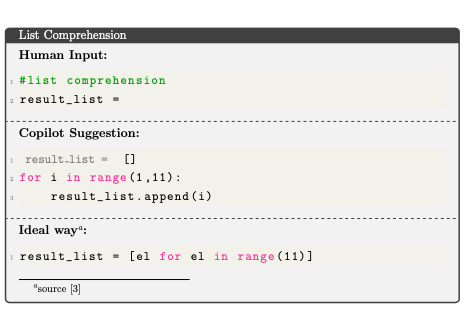
\includegraphics[width=\linewidth]{Figures/idioms_1.png}
    \caption{List Comprehension Idiom and Copilot Suggestion}
    \label{fig:idioms_1}
\end{figure}

The results show that Copilot did not suggest the optimal way as its first suggestion in the majority of the idioms we tested. This shows that current \cct{} like Copilot cannot suggest the idiomatic way in every suggestion even though they are the top most frequently used python idioms in public repositories on GitHub~\cite{Alexandru2018}. 

Copilot being closed source we cannot investigate the potential reasons behind this behavior. However, one plausible explanation for this behavior is that idiomatic ways may not be as frequent as non-idiomatic ways in Copilot's training data of public repositories on GitHub, making the non-idiomatic way rank higher than the idiomatic way.

\cct{} like Copilot should learn to detect idiomatic ways in public repositories and rank them higher than the most frequently used way in public repositories, so that the first suggestion would be the idiomatic way rather than the non-idiomatic way, which is the desirable way for \cct{} like Copilot. For the scope of this thesis, we leave resolving this problem as future work.

% \begin{tcolorbox}[title=List Comprehension,boxsep=.25mm]
%     %https://tex.stackexchange.com/questions/337909/tcolorbox-tcbline-style
% \textbf{Human Input:}
% \begin{lstlisting}[language={Python}]
% #list comprehension
% result_list = 
% \end{lstlisting}
% \tcbline
% \textbf{Copilot Suggestion:}
% \begin{lstlisting}[language=Python,escapechar=\%]
% % \noindent\textcolor{gray}{result\_list  =} % []
% for i in range(1,11):
%     result_list.append(i)
% \end{lstlisting}
% \tcbline
% \textbf{Idiomatic way\footnote{source \cite{Alexandru2018}}:}
% \begin{lstlisting}[language=Python]
% result_list = [el for el in range(11)]
% \end{lstlisting}
% \end{tcolorbox}

%%%%%% TODO: remember to update the screenshot if the source citation is different from the citation in the text %%%%%%

All the Idioms shown in Table~\ref{tab:all_idioms} can be found in the \repl{} including the code used as input (i.e., human input), the top suggestion by Copilot and the idiomatic way suggested in Alexandru et al.~\cite{Alexandru2018}.

\subsection{Code Smells}
\label{smells}
Using the methodology described in section~\ref{smells:methodology}, we sampled 10 best practices in javascript from AirBNB javascript coding style guide~\cite{airbnb_code} and compared Copilot syggestions when prompted with a input method(shown in section~\ref{smells:input}) and evaluated using methodology shown in section~\ref{smells:evaluation}. 

Copilot suggested the best practice from the coding guide for only one out of the ten coding standards we tested, i.e, 1 out of 10 instances Copilot had the recommended way as its top suggestion. Moreover, only 2 out of remaining 9 standards had the best practice in Copilot top 10 suggestions currently viewable. Copilot did not have the best practice in any of its top 10 suggestions for 7 standards out of 10 coding standards we tested.

% Copilot performed significantly worse than the Pythonic Idioms we showed in Section~\ref{secidioms}, As Copilot is closed source, we cannot find the reason behind this but one could argue that lack of data for JavaScript compared to python could be a reason for this behaviour. 

Table~\ref{tab:all_bp} shows the complete list of all the coding standards we tested on Copilot sampled from the AirBNB Coding Style guide~\cite{airbnb_code} and the ranking of the best practice in Copilot suggestions (if it exists).

\begin{table}[ht]
    \centering
    \begin{tabular}{|L|c|}
    \hline
         \textbf{Best Practice  Title} & \textbf{Copilot Suggestion Matched?} \\
         & (out of 10 suggestions) \\
         \hline
         Usage of Object method shorthand & No \\
         \hline
         Array Creating Constructor & 6\textsuperscript{th} \\
         \hline
         Copying Array Contents  & No \\
         \hline
         Logging a Function &  No \\
         \hline
         Exporting a Function & No \\
         \hline
         Sum of Numbers & 9\textsuperscript{th} \\
         \hline
         Accessing Properties & 1\textsuperscript{th} \\
         \hline
         Switch case usage & No \\
         \hline
         Return value from Function with a condition check & No \\
         \hline
         Converting Array-like object to an Array  & No \\
         \hline
    \end{tabular}
    \caption{List of all JavaScript Best Practices tested on Copilot.}
    \label{tab:all_bp}
\end{table}

Figure~\ref{fig:bp_1} shows the Best Practice for Copying Array Contents, showing user input (i.e., Human Input), the top suggestion by Copilot and the recommended way suggested by AirBNB JavaScript coding style guide~\cite{airbnb_code}.

\begin{figure}[hbt!]
    \centering
    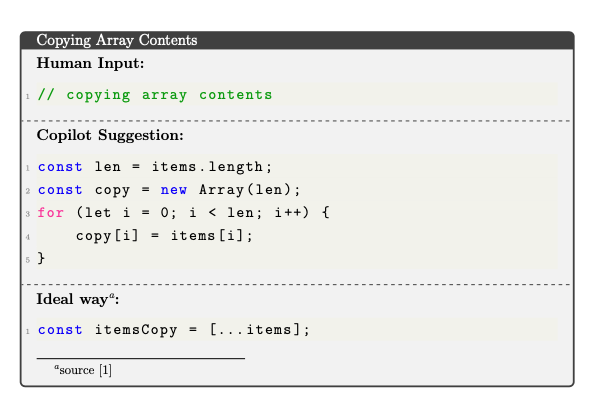
\includegraphics[width=\linewidth]{Figures/bp_1.png}
    \caption{Best Practice for Copying Array Contents and Copilot Suggestion.}
    \label{fig:bp_1}
\end{figure}

The results show that Copilot performed worse than the language idioms~(shown in chapter~\ref{chapter:idioms}). Copilot did not suggest the best practice as its first suggestion for 7 out of 10 coding standards we tested. This shows that current AI-supported
code completion tools like Copilot cannot suggest coding standards in its suggestions even though the coding standards are the sampled from widely accepted coding style guide.

All the Best Practices shown in Table~\ref{tab:all_bp} can be found in the \repl{} including the code used as input (i.e., human input), the top suggestion by Copilot and the best practice from AirBNB JavaScript coding style guide~\cite{airbnb_code}.

There could be many reasons for this performance like the public repositories do not always follow coding standards, Copilot cannot detect coding style from repositories that have contribution guides including the coding standards followed in the project. 
Copilot being closed source we cannot investigate the potential reasons behind this behavior and recommend ways to fix this issue improving the performance of Copilot.

We did not test Copilot for suggesting project specific coding styles because Copilot does not have the feature to customise its suggestions based on preferences~\cite{Copilot-web}.
However, \cct{} like Copilot should follow coding style guides and adapt their code suggestions to match the coding style used in the project. 
For example, if a user is working on a project where one of the coding style guideline says to leave a blank line after blocks and before the next statement~\cite{airbnb_code}. As a productivity tool, the ideal behaviour for \cct{} like Copilot is to detect the coding style guideline from existing code in the project and always suggest code that follows the guideline. 

% \begin{tcolorbox}[title=Copying Array Contents,boxsep=.15mm]
%     %https://tex.stackexchange.com/questions/337909/tcolorbox-tcbline-style
% \textbf{Human Input:}
% \begin{lstlisting}[language=JavaScript]
% // copying array contents
% \end{lstlisting}
% \tcbline
% \textbf{Copilot Suggestion:}
% \begin{lstlisting}[language=JavaScript]
% const len = items.length;
% const copy = new Array(len);
% for (let i = 0; i < len; i++) {
% 	  copy[i] = items[i];
% }
% \end{lstlisting}
% \tcbline
% \textbf{Ideal way\footnote{source \cite{airbnb_code}}:}
% \begin{lstlisting}[language=JavaScript]
% const itemsCopy = [...items];
% \end{lstlisting}
% \end{tcolorbox}

%%%%%% TODO: remember to update the screenshot if the source citation is different from the citation in the text %%%%%%


\subsection{Summary of Findings}
In an attempt to find the boundaries of \cct{} like Copilot, we analyzed Copilot code suggestions for Pythonic idioms and JavaScript best practices. 
We identified that Copilot did not suggest the idiomatic way as its top suggestion for 23 out of 25 coding scenarios in Python. 
Furthermore, we identified that Copilot did not suggest the recommended best practice for 22 out of 25 coding scenarios in JavaScript.

Although Copilot is very good at solving well-specified programming contest style problems~\cite{empirical_eval}, our experiments show that it does not do well in following idioms and recommending best practices in its code suggestions.
Additionally, \cct{} like Copilot being a productivity tool, should be able to suggest idiomatic approaches and recommended best practices in its code suggestions to be helpful for the user.
Studies like ours might help use this delineation to understand what might help turn \cct{} such as Copilot into full-fledged \AISE{} tools.
\section{Chapter Summary}
In summary, we start this chapter by showing the methodology used in addressing textbf{RQ-1} (What are the current boundaries of \cct{}?). 
We first introduced Pythonic idioms and best practices in JavaScript.
We then present our sampling approach for sampling 25 coding scenarios to analyze Copilot code suggestions.
Furthermore, we discussed the input given to Copilot to trigger a code suggestion 
and how the input was restricted to deriving the desired way from the input.
Finally, we described our evaluation approach for Copilot code suggestions.

We sampled 25 Pythonic idioms from Alexandru et al.~\cite{Alexandru2018}, and Farook et al.~\cite{idioms}.
We identified that Copilot did not suggest the idiomatic way as its top suggestion for 23 out of 25 coding scenarios in Python, which addressed \textbf{RQ-1.1} (How do \cct{} manage programming idioms?).
Furthermore, we sampled 25 best practices in JavaScript from the AirBNB JavaScript coding style guide~\cite{airbnb_code}. We identified that Copilot did not suggest the recommended best practice for 22 out of 25 coding scenarios in JavaScript, which addressed \textbf{RQ-1.2} (How do \cct{} manage to manage to suggest non-smelly code?).


% we showed that Copilot struggles to detect and most common idiomatic ways present in public repositories of GitHub and rank them higher than the non-idiomatic ways. The ideal behavior of \cct{} like Copilot in solving this problem is detecting common patterns present in code and rank them higher as the idiomatic ways for a task.
% In the next chapter (chapter~\ref{smells}), we look into how this ideal behavior can cause problems in the case of code smells, where common bad practices present in public repositories of GitHub can make \cct{} like Copilot introduce bad coding practices in its suggestions.

% % \section{Chapter Summary}
% In summary, we start this chapter by showing the methodology used in addressing \textbf{RQ-1.2} (How do \cct{} manage to suggest non-smelly code?). We first introduced the study setup with the input to Copilot and how it was restricted to deriving the best practice from the input and how the suggestions from Copilot were evaluated. We sampled best practices from AirBNB JavaScript coding style guide~\cite{airbnb_code}, and then compared it against Copilot suggestions. Based on results shown in Table~\ref{tab:all_bp}, Copilot struggles to suggest the best practices from widely used coding standards in its suggestions. 

In this chapter, we showed that Copilot struggles to detect and follow coding style guides present in public repositories of GitHub and always suggests code that follows those coding style guides. We also observed that Copilot struggles to detect and most common idiomatic ways present in public repositories of GitHub and rank them higher than the non-idiomatic ways. 
Identifying this delineation could help in urn AI-supported code completion tools such as Copilot into full-fledged AI-supported software engineering tools.
In the next chapter (chapter~\ref{chapter:framework}), we illustrate our taxonomy inspired by autonomous driving levels on the software abstraction hierarchy in \AISE{} and delineate where \cct{} like Copilot currently stands in the taxonomy. 